%% This is an example first chapter.  You should put chapter/appendix that you
%% write into a separate file, and add a line \include{yourfilename} to
%% main.tex, where `yourfilename.tex' is the name of the chapter/appendix file.
%% You can process specific files by typing their names in at the 
%% \files=
%% prompt when you run the file main.tex through LaTeX.
%% prompt when you run the file main.tex through LaTeX.
\chapter{Use of a Global Model to Understand Atmospheric Mercury Observations at Monitoring Sites in Latin America }\label{chapter2}
%% BACKGROUND
\begin{flushleft}
Environmental pollution from Hg damages ecosystems through Hg's transformation into toxic methylmercury and bio-accumulation in food chains. Further, Hg is highly mobile in the atmosphere, allowing it to travel to faraway places, resulting in worldwide distribution of its elemental form, \hg, which can last for as long as six months in the atmosphere\cite{horowitz_new_2017,shah_improved_2021}. Hg in the atmosphere can be classified as gaseous elemental Hg (GEM), gaseous oxidized Hg (GOM), and particulate-bound Hg (PBM)  \cite{lindberg_synthesis_2007,schroeder_atmospheric_1998,landis_development_2002}. In most cases, Hg emissions occur as gaseous elemental \hg, which is relatively inert and sparingly soluble in water \cite{horowitz_new_2017}. Since most Hg entering ecosystems comes from the atmosphere, monitoring and modeling atmospheric Hg and Hg deposition enables us to understand its biogeochemical cycle. In addition, a better understanding of Hg's circulation in the environment would enable effective policies to reduce its harmful effects.
\end{flushleft}
\section{Background}\label{chapter2_background}
\begin{flushleft}

Hg monitoring networks and atmospheric Hg models are closely interconnected in the literature. The study by Gustin et al.\cite{gustin_mercury_2020} where they describe modern scientific thinking regarding mercury in the environment, measurement methods, and how they relate to Minamata Convention on Mercury is a good example of this. Notably, the mutual dependency between atmospheric modeling and monitoring is presented in the MC's "Guidance on Monitoring Mercury and Mercury Compounds to Support the Effectiveness Evaluation of the Minamata Convention," which states that observations are needed not only to detect and quantify changes, but also to improve and evaluate models of mercury transport, fate, exposure, and impacts\cite{unep_guidance_2021}. Similarly, Sprovieri et al.\cite{sprovieri_atmospheric_2016} emphasize the importance of consistent global Hg measurements to validate regional and global-scale models.  According to Brasseur and Jacob\cite{brasseur_modeling_2017}, it is crucial to have a large ensemble of observations to evaluate atmospheric modeling outputs.
\end{flushleft}

\begin{flushleft}
Until now, no detailed model-observation comparison has been conducted for some world regions with high ASGM Hg emissions, such as Latin America or Africa. The lack of high-frequency atmospheric Hg monitoring capacity in these regions may have limited studies comparing observations to models in these regions, as shown in Figure \ref{fig:global-hg-monitoring-networks}, which illustrates the distribution of different Hg monitoring networks around the world as of the publication of the GMA 2018. It is evident in Figure \ref{fig:global-hg-monitoring-networks} that Latin America, Africa, and South East Asia remain significantly behind Europe and North America regarding access to large observation ensembles. 
\end{flushleft}

\begin{figure}[H]
  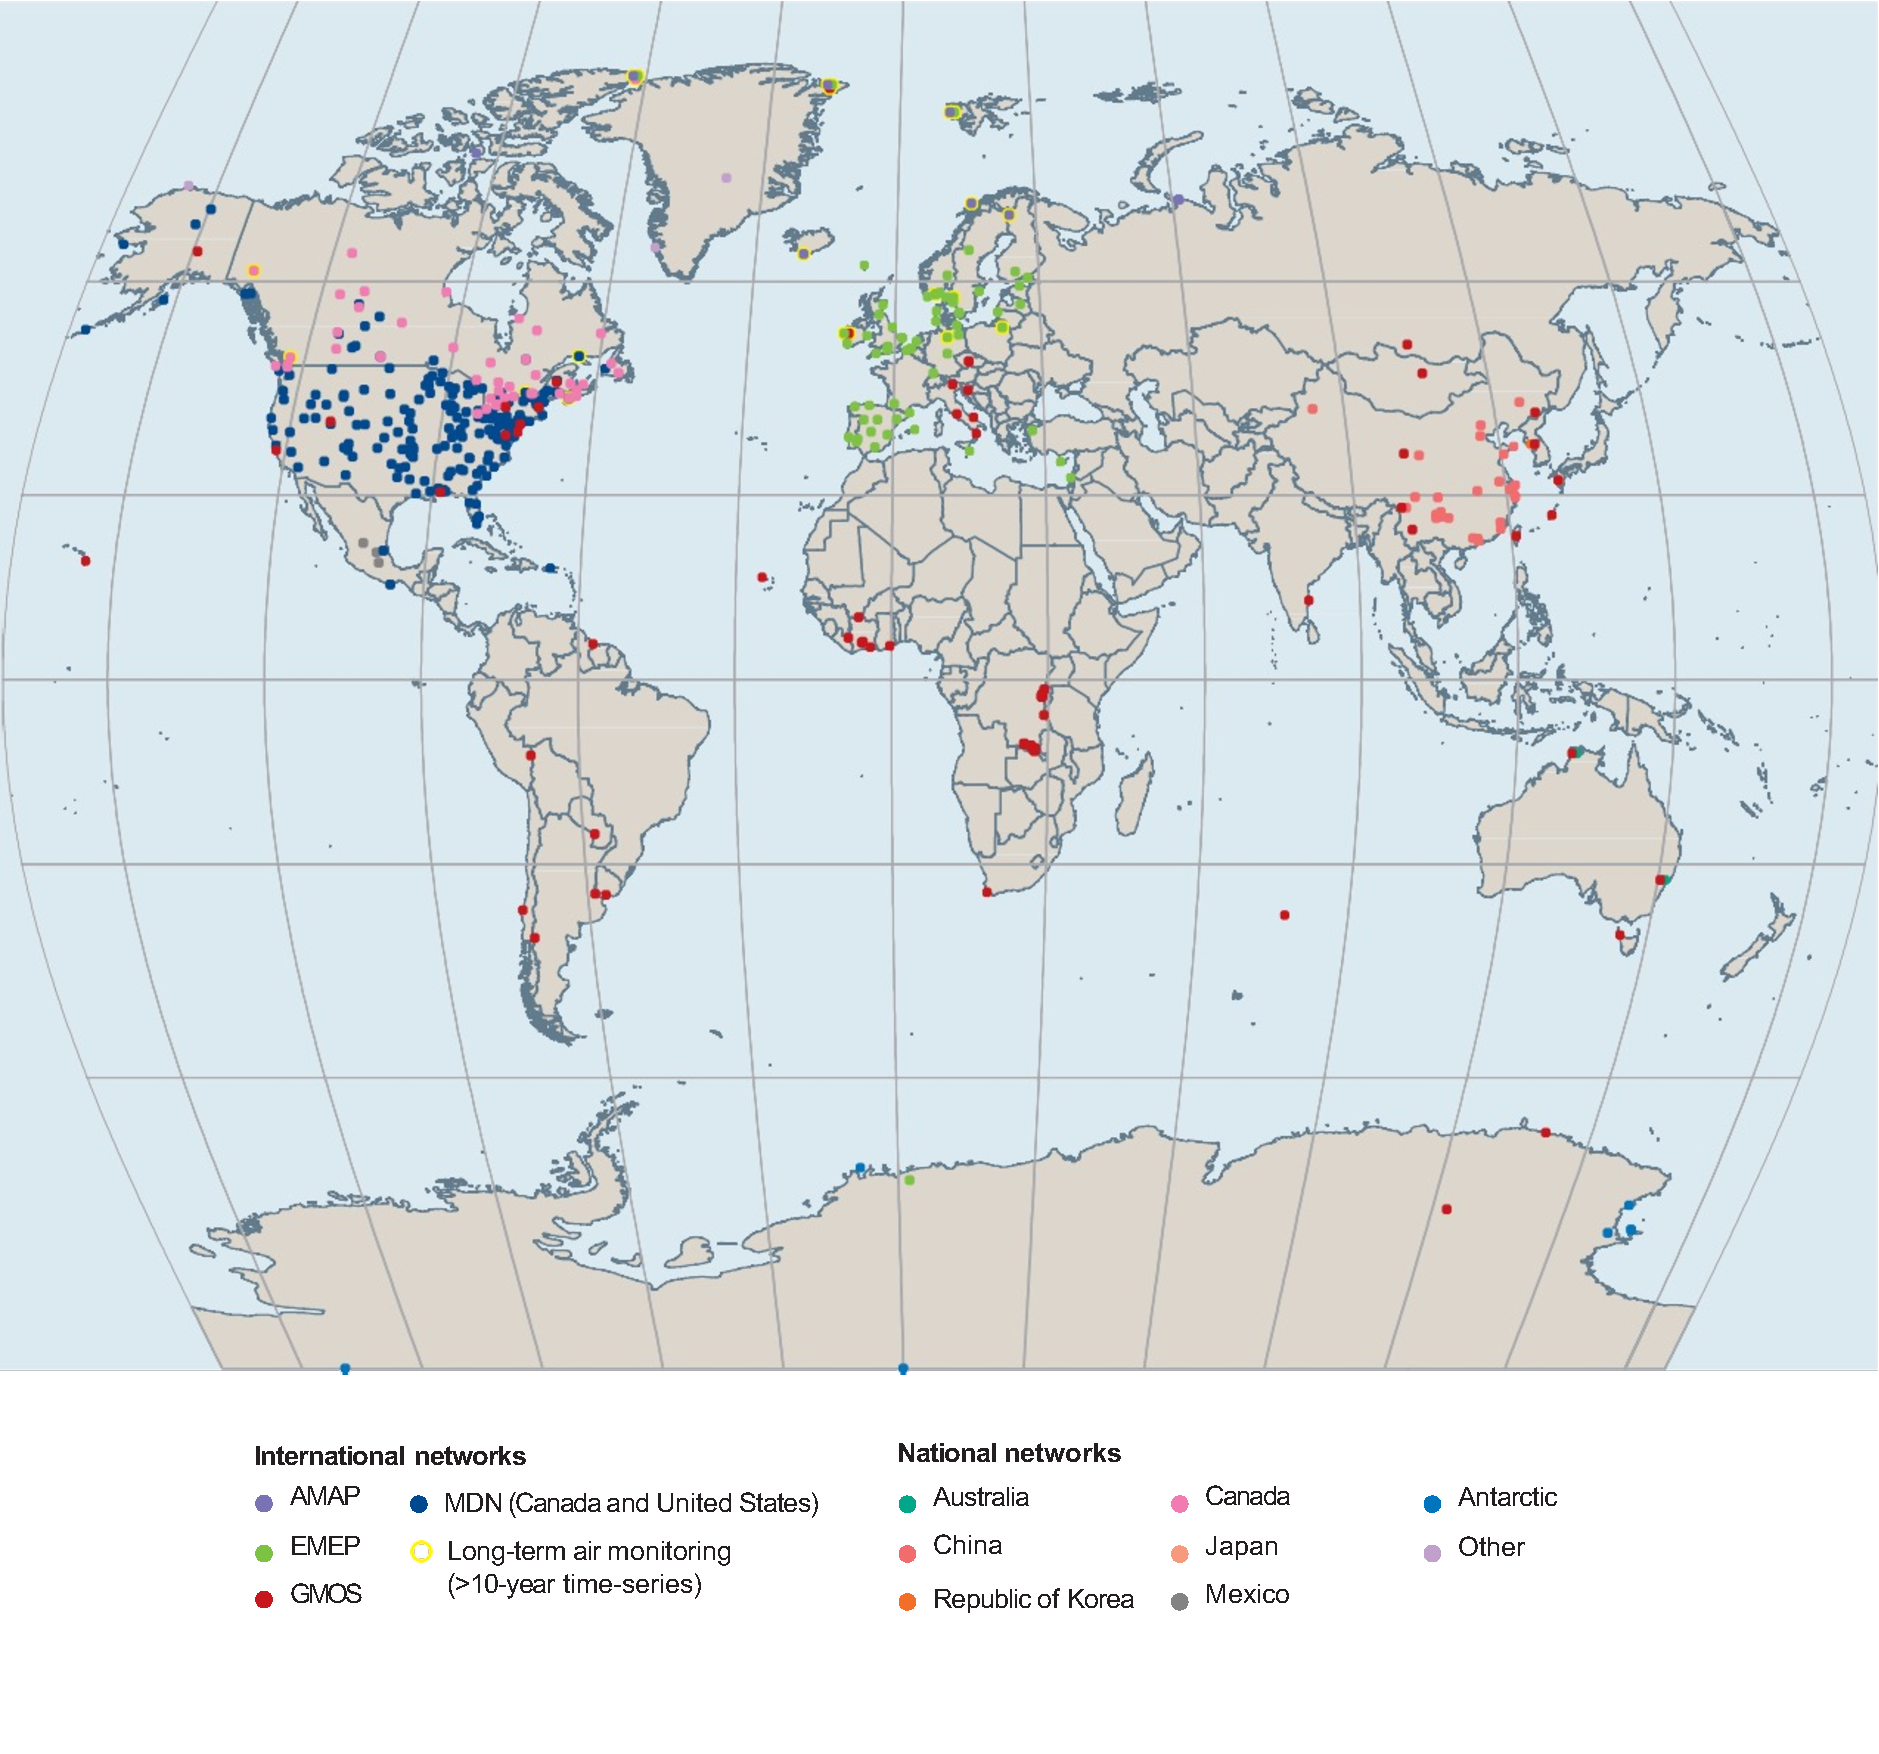
\includegraphics[width=\textwidth]{templates/figures/global-hg-monitoring-networks.pdf}
  \caption{Global map of Hg monitoring networks \cite{united_nations_environment_programme_technical_2019}}
  \label{fig:global-hg-monitoring-networks}
  \centering
  
\end{figure}
\FloatBarrier

\begin{flushleft}
 In this chapter, I compare outputs of the GEOS-Chem model with observed Hg at multiple sites in Latin America from two monitoring networks. I combine simulations of Hg in the atmosphere produced by the \gc CTM (Sect. \ref{c2_geos_chem_simulations}-Sect. \ref{c2_geos_chem_simulations}) with ground-based observations of atmospheric total gaseous mercury (TGM) (Sect. \ref{c2_monitoring_site_characteristics}) from the Global Mercury Observation System (GMOS)\cite{sprovieri_atmospheric_2016} and gaseous elemental mercury (GEM) data from a network of passive air samplers (PAS) distributed across Latin America. Then, I present comparisons between observations and model outputs and discuss the implications of the current state of atmospheric monitoring and modeling atmospheric Hg in Latin America(Sect. \ref{c2_results}). Finally, I summarize my conclusions (Sect. \ref{c2_conclusion}).
\end{flushleft}




%%----------------------------METHODS-------------------------------------------
\section{Methods}\label{c2_methods}
\subsection{GEOS-Chem Description}\label{c2_geos_chem_description}
\begin{flushleft}

The global atmospheric Hg concentration was simulated using version 12.8.1 of GEOS-Chem, whose Hg simulation is described by Horowitz et al.\cite{horowitz_new_2017}. All the simulations in this study were run globally for 47 vertical layers at a resolution of 2.0$\times$2.5, which is approximately equal to a 222 km$\times$277.5 km grid square at the equator \cite{horowitz_new_2017}. Moreover, the MERRA-2 assimilated meteorological data \cite{gelaro_modern-era_2017} drive the model's atmospheric transport, which calculates atmospheric Hg from three tracers: elemental Hg, Hg\textsuperscript{0}, divalent Hg, Hg\textsuperscript{2+}, and particulate-bound divalent Hg, Hg\textsuperscript{p}. The Hg chemical scheme in the GEOS-Chem version used in this study considers bromine (Br) to be the primary \hg oxidant\cite{horowitz_new_2017} and employs monthly mean Br oxidant concentrations from Schmidt et al.\cite{schmidt_modeling_2016}. 
\end{flushleft}

\begin{flushleft}

\subsection{GEOS-Chem Simulations}\label{c2_geos_chem_simulations}

The GMA 2018 emissions inventory was used to represent anthropogenic emissions sources from all sectors\cite{steenhuisen_development_2019}. Different inputs to the GEOS-Chem model, such as emissions sources, can be toggled on or off depending on the research objective; hence a reference simulation, \on was created by turning on all Hg emissions sources globally. Moreover, a \off was generated by turning off the ASGM source globally to evaluate the contribution of ASGM to the baseline modeled Hg$^0$ in the atmosphere by calculating the difference between the \on and \off. Table \ref{tab:geos_chem_simulation_description} describes the simulations that were conducted in detail.
\end{flushleft}

\begin{table}[H]
\captionof{table}{GEOS-Chem simulations conducted}
\label{tab:geos_chem_simulation_description}

\centering
\resizebox{\textwidth}{!}{\begin{tabular}{lccp{0.6\linewidth}}

\hline
Simulation Name &Period & Resolution & Description  \\
                        
\hline
Base (ASGM=ON)      & 2010-2016     & 2.0$\times$2.5 & All Hg anthropogenic emission sources are turned on  \\
No ASGM (ASGM=OFF)  & 2010-2016     & 2.0$\times$2.5 & All ASGM emissions are turned off\\
\hline
\end{tabular}}
\end{table}

\begin{flushleft}
 The frequency of the simulation output was set to output daily \hg averages at the global scale, while the \hg output for the grid boxes corresponding to the locations of the GMOS observation sites was set to an hourly frequency. The GEOS-Chem outputs for all the simulations were in units of parts per trillion (ppt) and were converted to \nang at standard temperature and pressure (273 K, 1 atm) to compare them to observations.
\end{flushleft}

\subsection{Monitoring Site Characteristics} \label{c2_monitoring_site_characteristics}
\begin{flushleft}
 The GMOS network is one of a few major global projects to develop a global observing system for mercury pollution. GMOS aims to provide high-quality Hg data sets in the Northern and Southern hemispheres to enable a more comprehensive assessment of atmospheric Hg concentrations and their dependence on meteorology, long-range atmospheric transport, and atmospheric emissions\cite{sprovieri_atmospheric_2016}. A vast network of ground-based monitoring stations, regular oceanographic cruises, and lower, upper, and stratospheric measurements make up this European Union-funded project \cite{koenig_seasonal_2021,sprovieri_atmospheric_2016}. More than 40 ground-based monitoring sites constitute the GMOS network, covering many regions with limited to no observational data before GMOS\cite{sprovieri_atmospheric_2016}. The GMOS monitoring network has five sites in Latin America that actively monitor Hg levels. Detailed analysis of the Sisal, Calhau, Manaus, Nieuw Nickerie and Bariloche sites was detailed in Sprovieri et al.\cite{sprovieri_atmospheric_2016}, and the Chalcataya site was analyzed in detail in Koenig et al.\cite{koenig_seasonal_2021}. A summary of the sites' characteristics is shown in Table \ref{tab:gmos_sites_info}. Moreover, the distribution of these GMOS sites in Latin America is indicated by the red triangles in Figure \ref{fig:Latam_Passive_SamplerSites}. 
 %A primary objective of this study was to evaluate the degree to which ASGM Hg emissions affected the Hg concentrations in the atmosphere at regional and global scales, so high-frequency GMOS data were collected to facilitate this evaluation.
  \end{flushleft}
  
  \begin{table}[H]
\captionof{table}{Cahracteristics of the GMOS sites evaluated \cite{koenig_seasonal_2021,sprovieri_atmospheric_2016}. }
\label{tab:gmos_sites_info}

\centering
\resizebox{\textwidth}{!}{\begin{tabular}{llccp{0.2\linewidth}rcll}
  \hline

Site                        & Site      & Latitude  & Longitude & Physical  & Elevation    & Number of      & Site &  Measurement  \\
                            & abbrev    &           &           &  Setting  & (m)           & Records (days) & Type&   Period \\
\hline
Sisal, Mexico               & SIS       & 21.16     & -90.05    &   Coastal site        &   7           &   320 &   Secondary    & 1/1/2010-1/1/2016   \\
Calhau, Cape Verde          & CAL       & 16.86     & -24.87    &   Coastal site        &   10          &   309 &   Secondary   & 1/1/2013-12/1/2014  \\
Nieuw Nickerie, Suriname    & NIK       & 5.93      & -56.98    &   Coastal site        &   1           &   215 &    Secondary   & 3/1/2007-12/1/2014 \\
Manaus, Brazil              & MAN       & -2.89     & -59.96    &    Amazon site       &  110          &   100 &   Master   & 1/1/2013-12/1/2014 \\
Chalcataya, Bolivia         & CHC       & -16.2     & -68.12    &    Mountain site       &  5340         &   333 &    Secondary   & 7/1/2014-2/1/2016  \\
Bariloche, Agentina         & BAR       & -41.13    & -72.42    &    Mountain site       &  800          &   333 &  Master     & 10/1/2012-7/1/2017 \\
  \hline
\end{tabular}}

\end{table}

  
 \begin{flushleft}
  The GMOS sites are classified as either secondary or master sites in Table\ref{tab:gmos_sites_info} to indicate the type of data collected and the type of equipment used at the site. The secondary sites used the Tekran continuous mercury vapor analyzer, model 2537A/B (Tekran Instruments Corp., Toronto, Ontario, Canada), except for the Nieuw Nickerie site (NIK), Suriname, which used a Lumex RA-915+ mercury analyzer. The master sites used the Tekran model 2537A/B mercury vapor analyzer coupled with their speciation system model 1130 for GOM and model 1135 for particulate boundaries mercury (PBM2.5) with fractions less than 2.5 $\mu$m in diameter to prevent large particles from depositing on the KCl-coated denuder \cite{koenig_seasonal_2021,sprovieri_atmospheric_2016,gustin_measuring_2015}
\end{flushleft}


\begin{figure}[H]
 \centering
  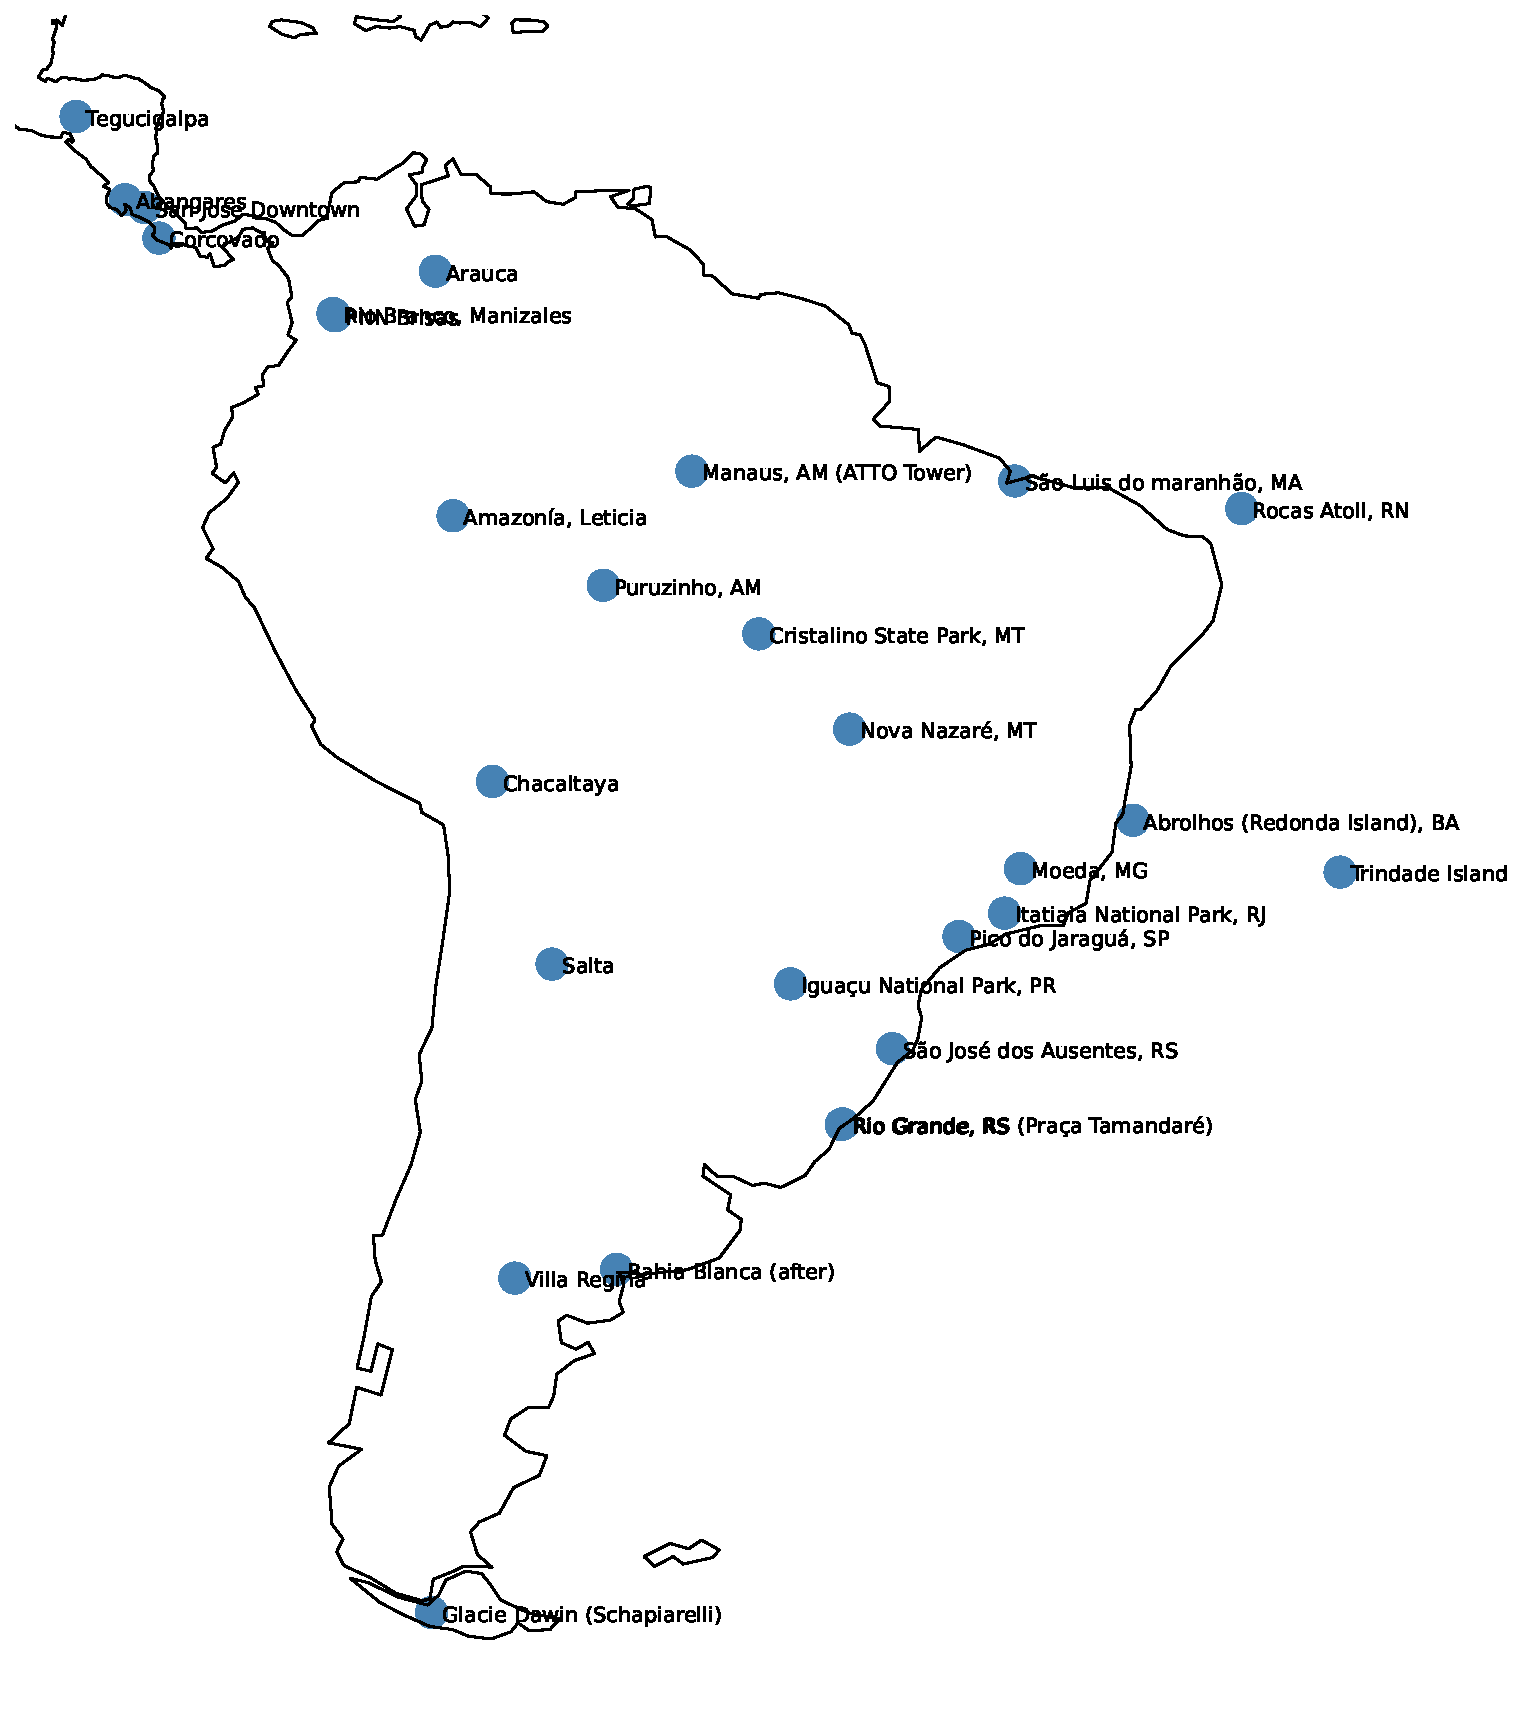
\includegraphics[width=0.8\textwidth]{templates/figures/Passive_Samplers/Latam_Passive_SamplerSites.pdf}
  \caption{Map showing the names and locations of the GMOS Monitoring Network Sites and Passive Sampler sites in Latin America. GMOS sites are indicated by the red triangles, and the PAS sites are indicated by the blue dots\cite{quant_measuring_2021,koenig_seasonal_2021}.}
  \label{fig:Latam_Passive_SamplerSites}
\end{figure}
\FloatBarrier

\begin{flushleft}
    In contrast to active Hg monitoring equipment used in the GMOS network, which can be prohibitively expensive, energy-intensive, and require extensive training, passive air samplers (PAS) require no energy to operate and do not require any special handling skills \cite{quant_measuring_2021}. Furthermore, PAS can be easily deployed for long periods. This combination of attributes of PAS allows more sampling sites to be studied over extended periods enabling significant average GEM concentration estimates to be obtained. PAS monitoring is integral in informing the effectiveness evaluation of the MC\cite{gustin_measuring_2015,unep_guidance_2021}. Quant (2021) published a detailed analysis of the PAS sites in Latin America, and their respective locations are shown by the blue circles in Figure \ref{fig:Latam_Passive_SamplerSites}. 
\end{flushleft}

\subsection{Pre-processing and Comparison of Observed and Modeled Mercury Concentration in the Atmosphere}\label{c2_observation_data_manipulation}
\begin{flushleft}
  The average annual GEM concentration data for 27 PAS sites in Latin America was obtained from Quant et al.\cite{quant_measuring_2021}, which included information about the coordinates of the deployment sites and the period of measurement. The PAS data was already \nang hence there was no need for pre-processing before comparison with the modeled concentrations. Available Hg observation data from the GMOS stations on Figure  \ref{fig:Latam_Passive_SamplerSites} was obtained from the GMOS online database (http://www.gmos.eu), as well as published studies about the Hg monitoring data from the different sites  \cite{koenig_seasonal_2021}. The data sets were pre-processed based on the information in Sprovieri et al.,(2016) and Koenig et al.,(2021) and daily and annual averages to compare with the \gc output\cite{koenig_seasonal_2021,sprovieri_atmospheric_2016}. The PAS data was compared to the modeled annual average Hg concentration for 2015 to evaluate, and the coordinate information from the PAS data was used to directly compare the GEM observations and model outputs at the respective PAS sites.
\end{flushleft}





%%----------------------------RESULTS AND DISCUSSION---------------------------
\section{Results and Discussion}\label{c2_results}

\begin{figure}[H]
\centering
  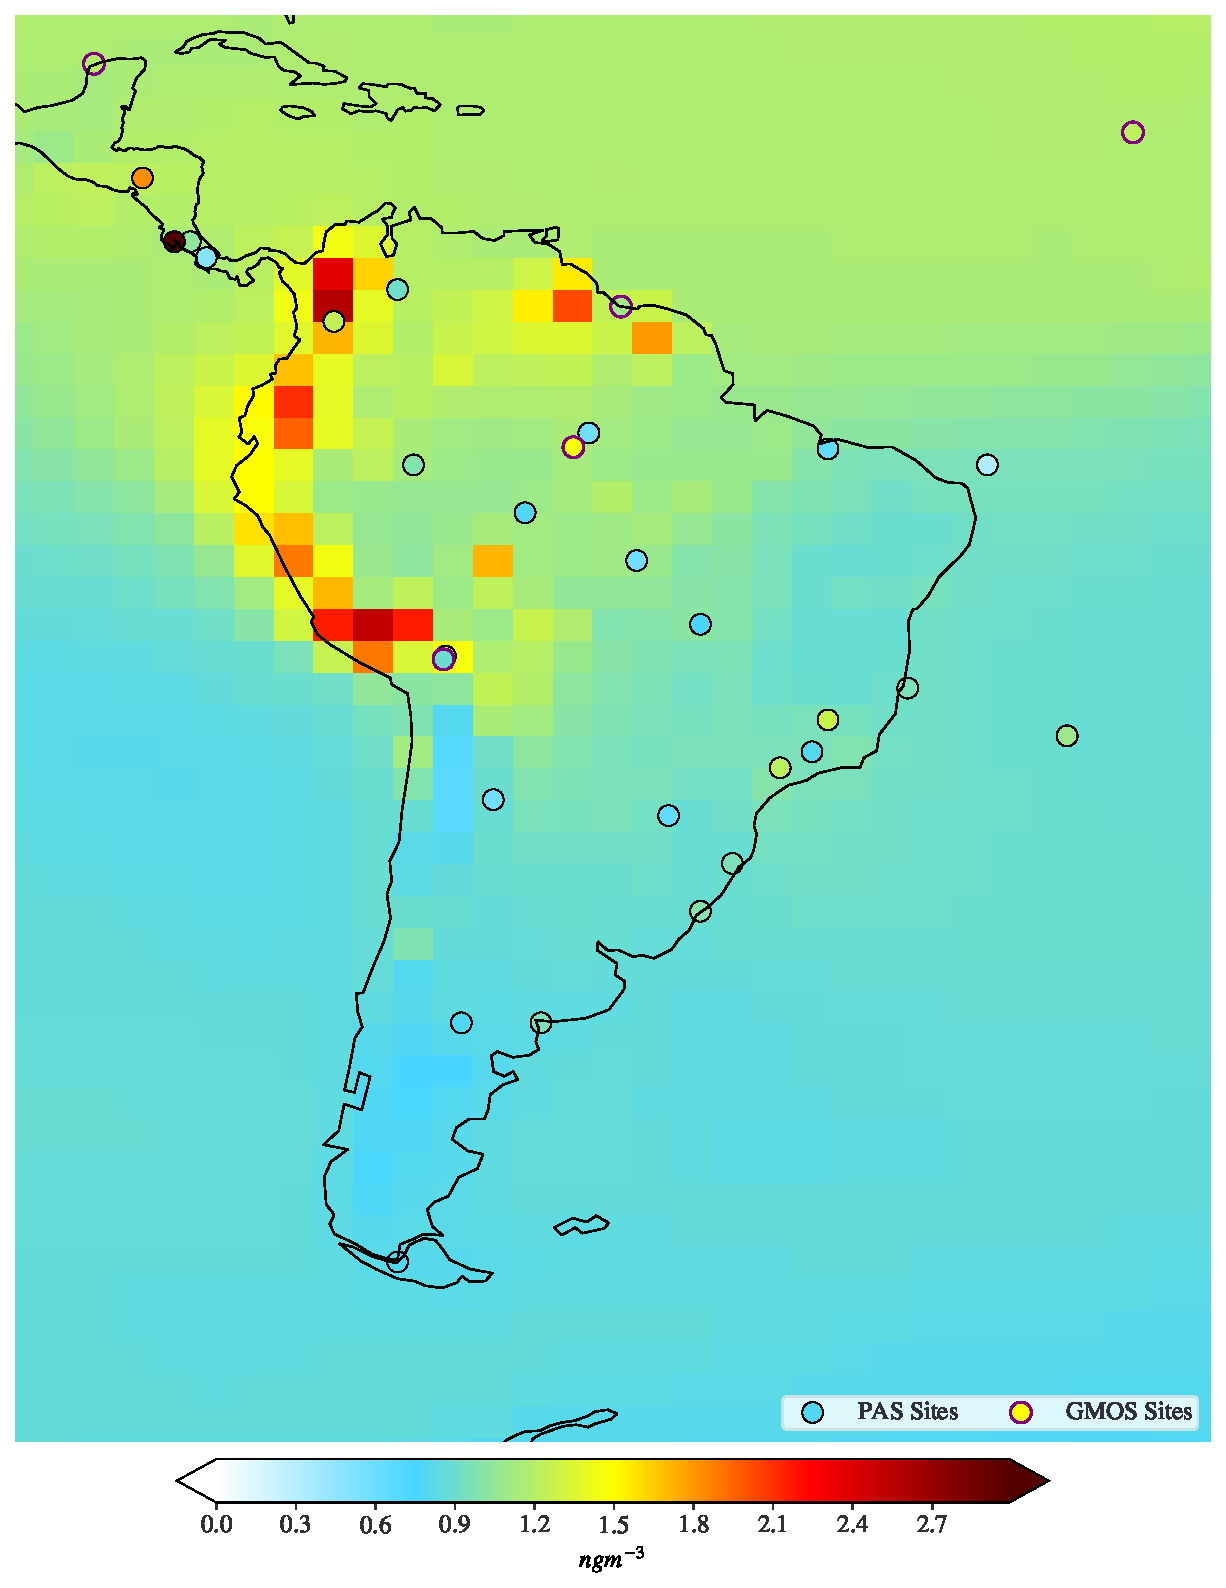
\includegraphics[width=0.7\textwidth]{templates/figures/Passive_Samplers/07-27-22_pas_vs_model_Hg0-per-year_001.pdf}
  \caption{Annual average Hg concentration on the surface in Latin America averaged. The background is the annual average \hgc produced by the \on for 2015. The circles are the annual average GEM concentration from the PAS sites, while the triangles are the annual average TGM concentrations from the GMOS sites.\cite{quant_measuring_2021,sprovieri_atmospheric_2016,koenig_seasonal_2021}}
  \label{fig:06-12-22_pas_vs_model_Hg0-per-year_001}
  
  
\end{figure}
\FloatBarrier
\begin{flushleft}
 Recent publications analyzing global Hg monitoring data highlight an observed interhemispheric gradient of Hg where Hg concentration in the southern hemisphere is lower than Hg concentration in the northern hemisphere\cite{sprovieri_atmospheric_2016}. This gradient is evident in the simulated background annual average \hg concentration as seen in Figure \ref{fig:06-12-22_pas_vs_model_Hg0-per-year_001}. Moreover, most GMOS sites validate the modeled interhemispheric gradient. Seemingly, the model matches the PAS GEM measurement at Chalcataya but, according to Quant et al. 2021, the higher GEM levels observed at Chacaltaya (1.4 ng m-3) are likely to reflect a known Hg spill near the sampling site and may not reflect regional values\cite{quant_measuring_2021}. In comparison with PAS data, the GEOS-Chem model overestimates atmospheric concentrations. This phenomenon is more prevalent in inland sites than coastal ones. In the Amazon region, for example, there is a difference between the model and inland PAS sites. This may be because the GEOS-Chem model used in this study underestimates Hg uptake by plants \cite{feinberg_evaluating_2022}. 
\end{flushleft}
\begin{flushleft}
 
 Figure \ref{fig:06-12-22_pas_vs_model_Hg0-per-year_by-latitude_001} which shows the modeled (blue circles) and observed (red circles) annual average \hg plotted as a function of latitude indicates the interhemispheric gradient observed in GEOS-Chem. The observation error bars represent the replicate precision of the observations, while the model error bars represent the \nft bootstrap confidence interval for the mean annual \hg. 
\end{flushleft}
 
\begin{figure}[H]
  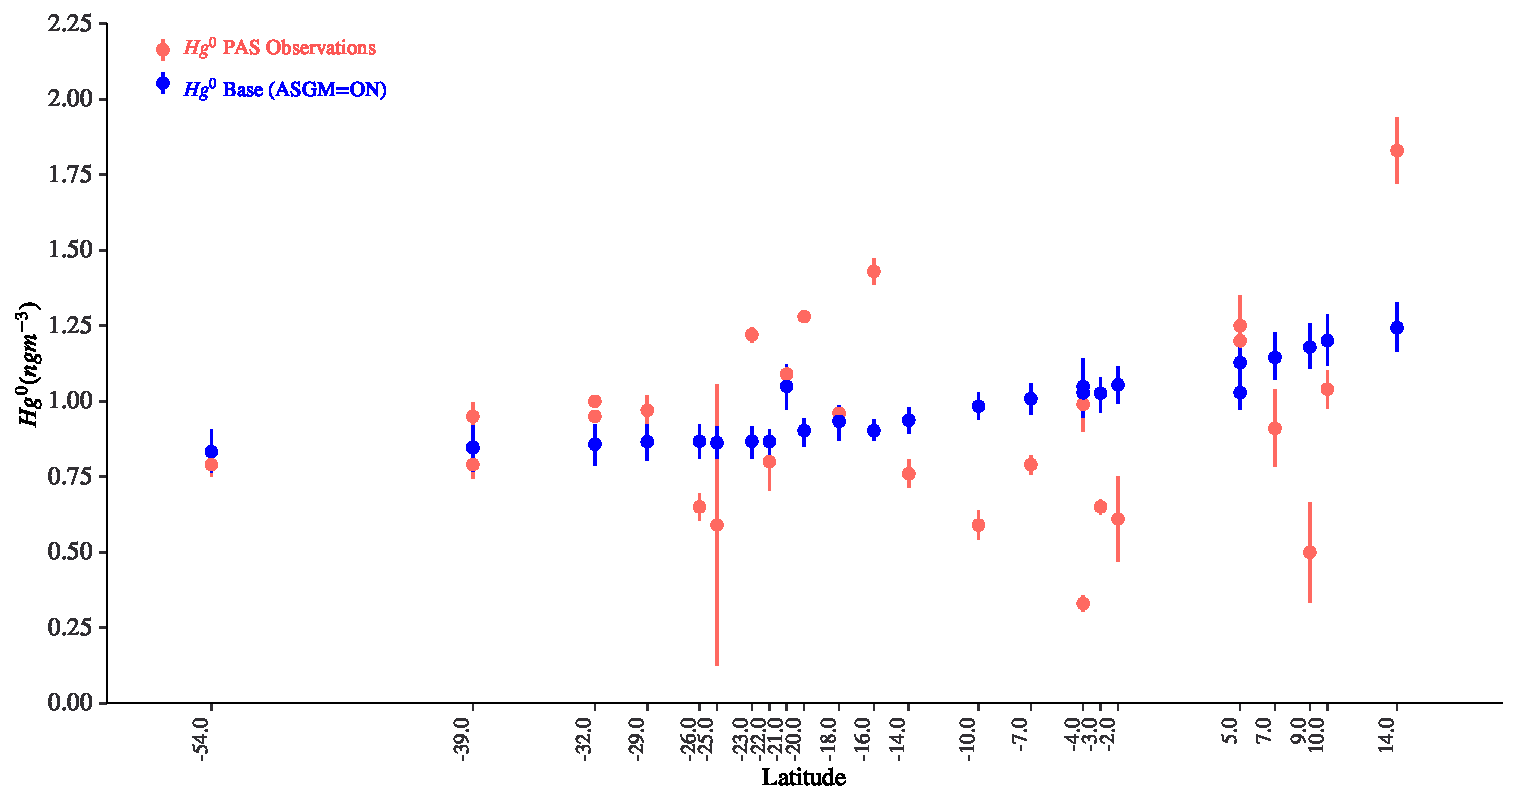
\includegraphics[width=\textwidth]{templates/figures/Passive_Samplers/06-12-22_pas_vs_model_Hg0-per-year_by-latitude_001.pdf}
  \caption{\hg in the atmosphere as a function of Latitude. The \on (blue circles) and observed (red circles) annual average \hg plotted are plotted as a function of latitude to evaluate spatial trends across the continent. The observation error bars represent the replicate precision of the observations while the model error bars represent the 95\textsuperscript{th} bootstrap confidence interval for the mean annual \hg.}
  \label{fig:06-12-22_pas_vs_model_Hg0-per-year_by-latitude_001}
  \centering
  
\end{figure}
\FloatBarrier
\begin{flushleft}
    \gcs overestimation of Hg concentration in the Amazon region observed above was also addressed in Feinberg et al. (2022), who compared simulations with litterfall, throughfall, and flux tower measurements from 93 forested sites to evaluate vegetation as a Hg sink. According to their results, the \gc version, 12.8 underestimates \hg dry deposition, which may explain why measurements of Hg concentration in Latin America were lower than predicted by \gc. 

\end{flushleft}

\subsection{Modeled vs. Observed Temporal Trends}\label{c2_modeled_vs_observed_trends}
\begin{figure}[H]
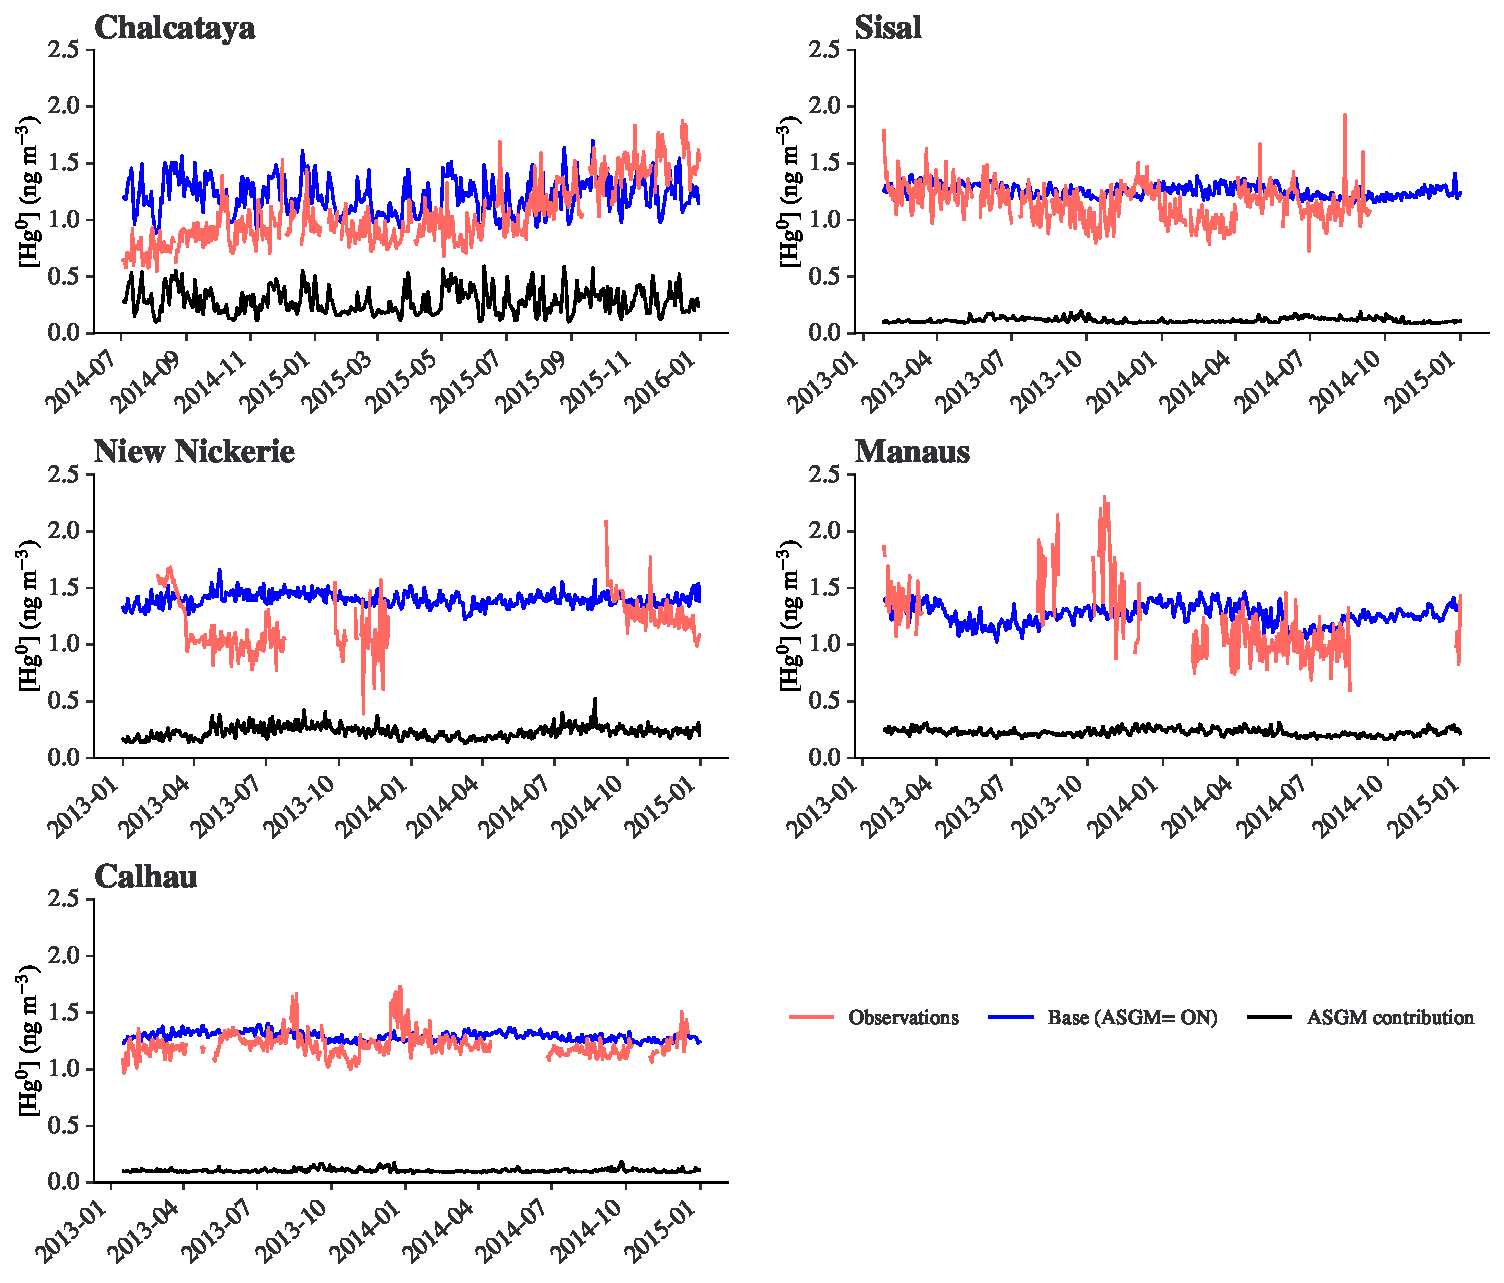
\includegraphics[width=\textwidth]{templates/figures/GMOS_Sites/GMOS_Sites.pdf}
\centering
\captionof{figure}{Time series plots of the observed TGM concentrations at different GMOS sites in red with the corresponding modeled concentration in blue and the associated ASGM contribution in green. Except for the CHC site, where the data are from July 2014 and January 2016, the available data and corresponding model outputs were plotted between January 2013 and January 2016.}
\label{fig:GMOSvsGC}
\end{figure}
\FloatBarrier


\begin{flushleft}


 This study also compared observed and modeled data on a daily resolution as seen in Figure \ref{fig:GMOSvsGC}, which shows the time series of the modeled \hgc in the atmosphere alongside the observed Hg and the simulated ASGM contribution to the atmospheric Hg concentration at the GMOS sites. The \gc model version used in this study overestimated the concentration of Hg on most days. However, the \gc estimated average \hgc over the available observation period was within one standard deviation of the observed Hg in most of the sites except for the Manaus and Nieuw Nickerie sites. \gcs overestimates the observed GEM concentrations at the Manaus and Bariloche master sites by over 25\%  and the GEM concentration at Nieuw Nickerie by 20\%, which may be indicative of poor parameterization of GEM in the model. Moreover, the overestimation of GEM concentrations in Manaus further indicates the model's poor implementation of Hg plant uptake through dry deposition, as discussed in Feinberg et al.(2022)\cite{feinberg_evaluating_2022}.
\end{flushleft}


\begin{figure}[H]
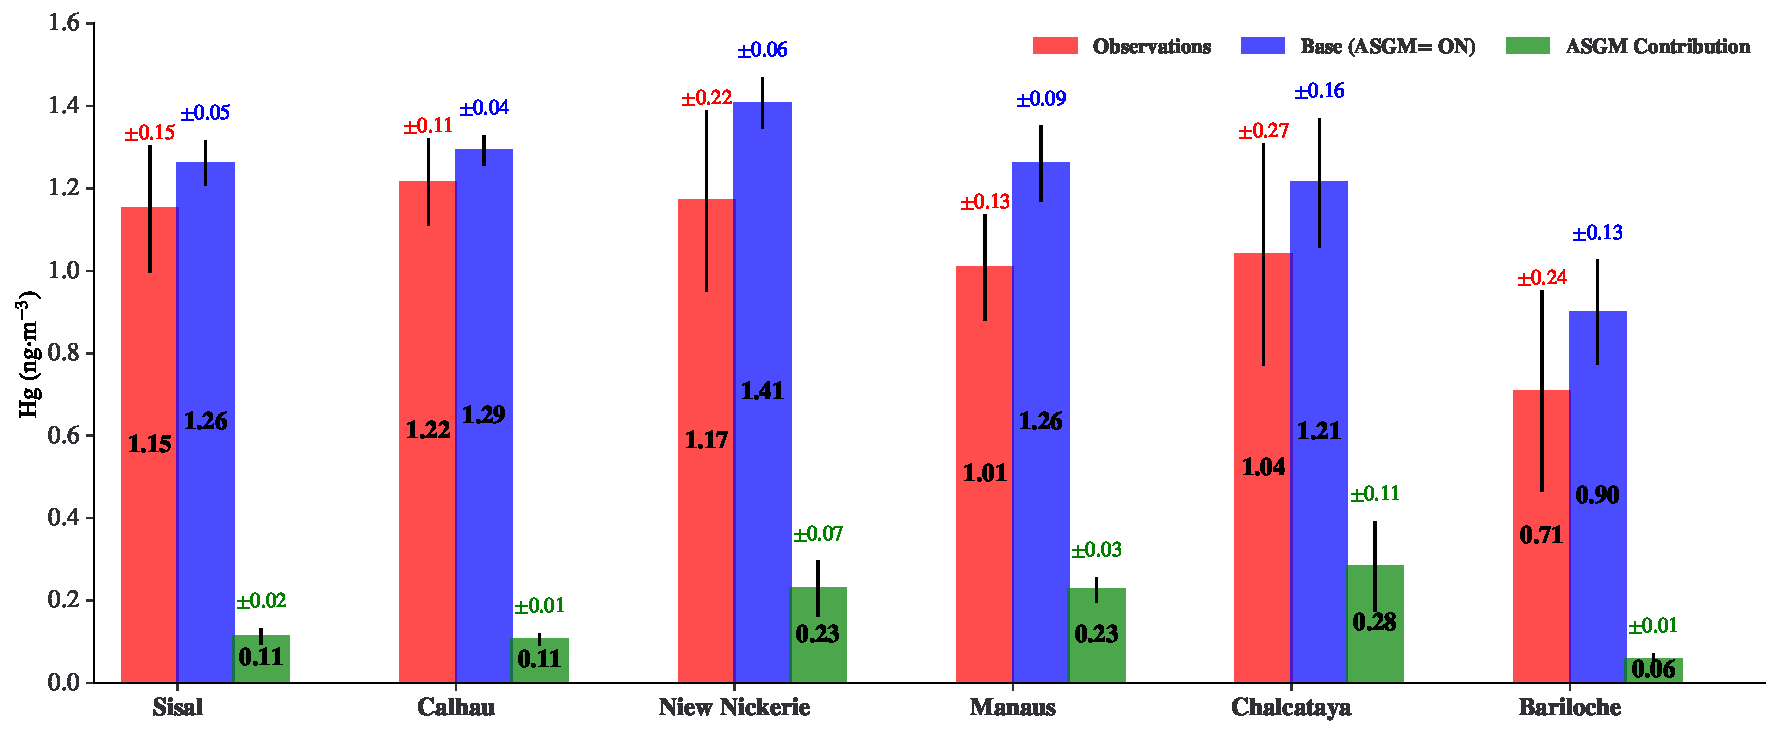
\includegraphics[width=\textwidth]{templates/figures/GMOS_Sites/gmos_sites_stats.pdf}
\centering
\captionof{figure}{Bar chart comparing the modeled and observed average Hg concentration at the respective GMOS Sites. The bars are annotated with the average Hg concentration values. Moreover, the error bars and the annotated value above the bars show the standard deviation in each data set. }
\label{fig:gmos_sites_stats}
\end{figure}
\FloatBarrier

\begin{flushleft}
Moreover, Figure \ref{fig:GMOSvsGC} and Figure \ref{fig:gmos_sites_stats} clearly show that ASGMs modeled contribution is low in most sites except for Chacaltaya, Manaus, and Nieuw Nickerie. The model's behavior regarding the predicted ASGM contribution at these sites is not surprising since these sites are in countries estimated to be among the top 10 Latin American ASGM Hg emitters in the ASGM emission inventory used for \gc simulation. Even though the model estimates a notable ASGM contribution at the Manaus (18\%) and Nieuw Nickerie (16\%) sites, the sites lack enough data to fully characterize the ASGM contribution to the Hg concentration over the long term. However, the predicted  ASGM Hg contribution at Chacaltaya is the highest at 23\% as seen in Table \ref{tab:model_percentage_overestimation_of_mean}. 
\end{flushleft}

\begin{table}[H]
\captionof{table}{Table showing the extent to which the model predicts the observations showed by the percentage difference between the model predictions and the observations }
\label{tab:model_percentage_overestimation_of_mean}

\center
\resizebox{\textwidth}{!}{\begin{tabular}{lcccc}
  \hline

GMOS Site       & Observed Average TGM/GEM  & Modeled Average \hg        &  Percentage difference between       &   Percentage ASGM\\
                &  Concentration (\nang )   &  Concentration (\nang)     &  modeled and observed average (\%)   &   Contribution (\%) \\
                        
\hline
Sisal          &     1.15               &             1.26               & 10                                   & 9 \\
Calhau         &     1.22               &             1.29               & 6                                    & 9 \\
Nieuw Nickerie &     1.17               &             1.41               & 20                                   & 16\\
Manaus         &     1.01               &             1.26               & 25                                   & 18 \\
Chalcataya     &     1.04               &             1.21               & 17                                   & 23 \\
Bariloche      &     0.71               &             0.9                & 27                                   & 6 \\
  \hline
\end{tabular}}
\end{table}


\begin{flushleft}
 Correlations across the time series in Fig.\ref{fig:GMOSvsGC} between observations and the model are shown in Fig. \ref{fig:gmos_sites_scatter}. The general observation is that model poorly matched the observations (mild and even flat slope)  and shallow $r^2$ values. The low correlations between the model and observations may be attributed to poor vegetation uptake, which has already been discussed\cite{feinberg_evaluating_2022}. Moreover, the poor parameterizations of emissions in the model may reduce the extent to which the model recreates the observed atmospheric Hg concentrations. Chapter 3 will investigate the emission parameterizations further to determine how and why the model's input of ASGM emissions is poor. 
\end{flushleft}
 \begin{figure}[H]
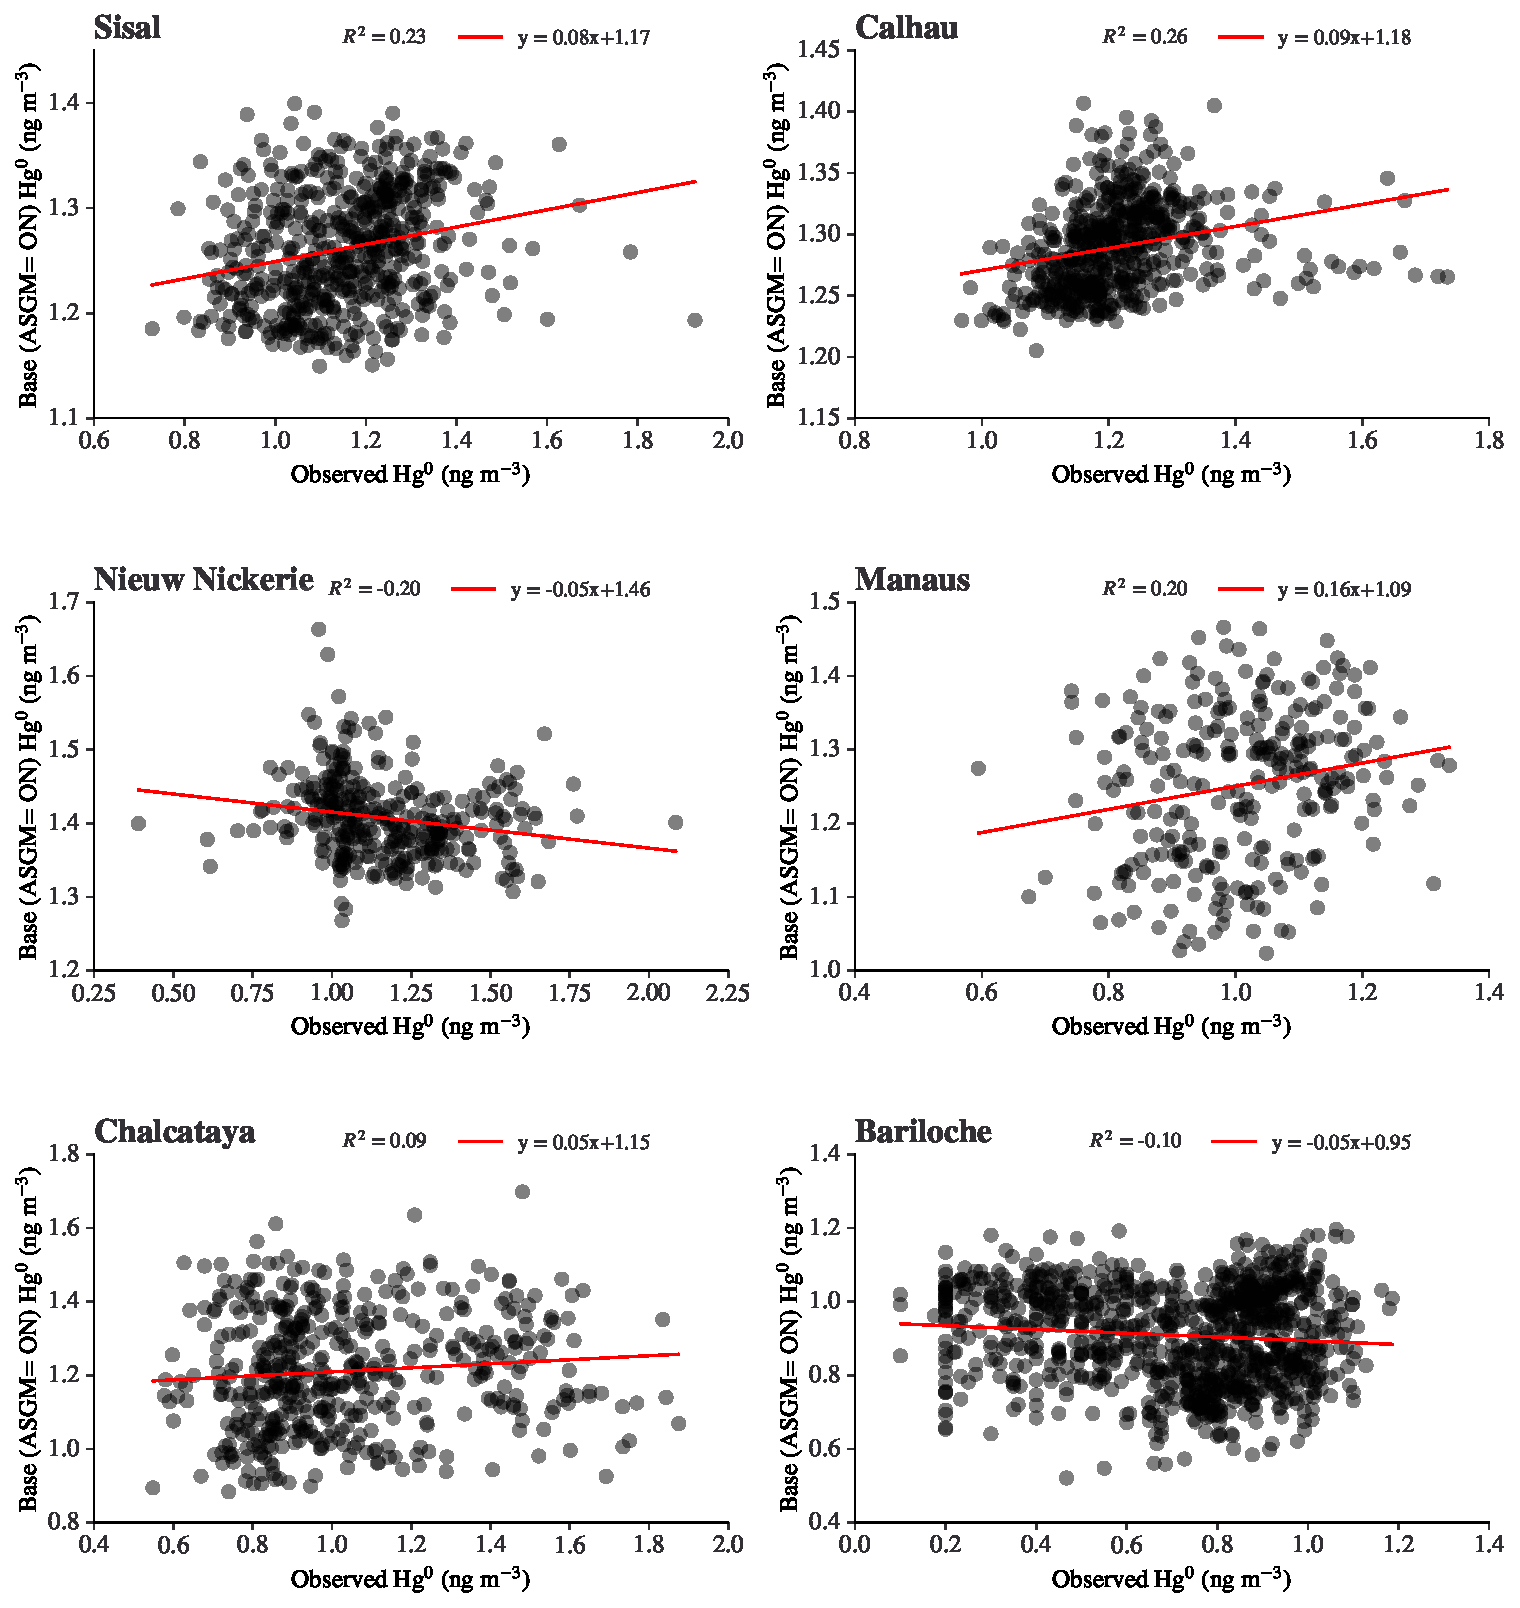
\includegraphics[width=\textwidth]{templates/figures/GMOS_Sites/gmos_sites_scatter.pdf}
\centering
\captionof{figure}{Scatter plots of the modeled Hg concentration as a function of the observed concentration. The red line is used to investigate the extent of the linear relationship between the modeled and observed Hg concentrations}
\label{fig:gmos_sites_scatter}
\end{figure}
\FloatBarrier


\section{Conclusion}\label{c2_conclusion}

\begin{flushleft}
For this study, we compiled the atmospheric Hg measurements from six GMOS sites across Latin America discussed in \cite{koenig_seasonal_2021,sprovieri_atmospheric_2016}. Additionally, we gathered annual average GEM measurements from 27 PAS sites across Latin America, published in Quant et al.(2021). These data on the measured atmospheric GEM and TGM concentration in Latin America were compared with \hgc simulated by the GEOS-Chem global Hg model with the oxidation scheme explained in Horowitz et al. (2017) to examine spatiotemporal trends and test for evidence of ASGM contributions to measured Hg. A relatively weak relationship was found between the observed mercury species (GEM and TGM) and those in the \on, demonstrating a need for an improved understanding of fundamental chemistry in the \gc model.

\end{flushleft}